\documentclass[twoside]{book}

% Packages required by doxygen
\usepackage{fixltx2e}
\usepackage{calc}
\usepackage{doxygen}
\usepackage[export]{adjustbox} % also loads graphicx
\usepackage{graphicx}
\usepackage[utf8]{inputenc}
\usepackage{makeidx}
\usepackage{multicol}
\usepackage{multirow}
\PassOptionsToPackage{warn}{textcomp}
\usepackage{textcomp}
\usepackage[nointegrals]{wasysym}
\usepackage[table]{xcolor}

% Font selection
\usepackage[T1]{fontenc}
\usepackage[scaled=.90]{helvet}
\usepackage{courier}
\usepackage{amssymb}
\usepackage{sectsty}
\renewcommand{\familydefault}{\sfdefault}
\allsectionsfont{%
  \fontseries{bc}\selectfont%
  \color{darkgray}%
}
\renewcommand{\DoxyLabelFont}{%
  \fontseries{bc}\selectfont%
  \color{darkgray}%
}
\newcommand{\+}{\discretionary{\mbox{\scriptsize$\hookleftarrow$}}{}{}}

% Page & text layout
\usepackage{geometry}
\geometry{%
  a4paper,%
  top=2.5cm,%
  bottom=2.5cm,%
  left=2.5cm,%
  right=2.5cm%
}
\tolerance=750
\hfuzz=15pt
\hbadness=750
\setlength{\emergencystretch}{15pt}
\setlength{\parindent}{0cm}
\setlength{\parskip}{3ex plus 2ex minus 2ex}
\makeatletter
\renewcommand{\paragraph}{%
  \@startsection{paragraph}{4}{0ex}{-1.0ex}{1.0ex}{%
    \normalfont\normalsize\bfseries\SS@parafont%
  }%
}
\renewcommand{\subparagraph}{%
  \@startsection{subparagraph}{5}{0ex}{-1.0ex}{1.0ex}{%
    \normalfont\normalsize\bfseries\SS@subparafont%
  }%
}
\makeatother

% Headers & footers
\usepackage{fancyhdr}
\pagestyle{fancyplain}
\fancyhead[LE]{\fancyplain{}{\bfseries\thepage}}
\fancyhead[CE]{\fancyplain{}{}}
\fancyhead[RE]{\fancyplain{}{\bfseries\leftmark}}
\fancyhead[LO]{\fancyplain{}{\bfseries\rightmark}}
\fancyhead[CO]{\fancyplain{}{}}
\fancyhead[RO]{\fancyplain{}{\bfseries\thepage}}
\fancyfoot[LE]{\fancyplain{}{}}
\fancyfoot[CE]{\fancyplain{}{}}
\fancyfoot[RE]{\fancyplain{}{\bfseries\scriptsize Generated by Doxygen }}
\fancyfoot[LO]{\fancyplain{}{\bfseries\scriptsize Generated by Doxygen }}
\fancyfoot[CO]{\fancyplain{}{}}
\fancyfoot[RO]{\fancyplain{}{}}
\renewcommand{\footrulewidth}{0.4pt}
\renewcommand{\chaptermark}[1]{%
  \markboth{#1}{}%
}
\renewcommand{\sectionmark}[1]{%
  \markright{\thesection\ #1}%
}

% Indices & bibliography
\usepackage{natbib}
\usepackage[titles]{tocloft}
\setcounter{tocdepth}{3}
\setcounter{secnumdepth}{5}
\makeindex

% Hyperlinks (required, but should be loaded last)
\usepackage{ifpdf}
\ifpdf
  \usepackage[pdftex,pagebackref=true]{hyperref}
\else
  \usepackage[ps2pdf,pagebackref=true]{hyperref}
\fi
\hypersetup{%
  colorlinks=true,%
  linkcolor=blue,%
  citecolor=blue,%
  unicode%
}

% Custom commands
\newcommand{\clearemptydoublepage}{%
  \newpage{\pagestyle{empty}\cleardoublepage}%
}

\usepackage{caption}
\captionsetup{labelsep=space,justification=centering,font={bf},singlelinecheck=off,skip=4pt,position=top}

%===== C O N T E N T S =====

\begin{document}

% Titlepage & ToC
\hypersetup{pageanchor=false,
             bookmarksnumbered=true,
             pdfencoding=unicode
            }
\pagenumbering{roman}
\begin{titlepage}
\vspace*{7cm}
\begin{center}%
{\Large P\+A04 }\\
\vspace*{1cm}
{\large Generated by Doxygen 1.8.11}\\
\end{center}
\end{titlepage}
\clearemptydoublepage
\tableofcontents
\clearemptydoublepage
\pagenumbering{arabic}
\hypersetup{pageanchor=true}

%--- Begin generated contents ---
\chapter{Hierarchical Index}
\section{Class Hierarchy}
This inheritance list is sorted roughly, but not completely, alphabetically\+:\begin{DoxyCompactList}
\item \contentsline{section}{Event}{\pageref{struct_event}}{}
\item \contentsline{section}{Event\+Queue}{\pageref{class_event_queue}}{}
\begin{DoxyCompactList}
\item \contentsline{section}{A\+B\+Event\+Queue}{\pageref{class_a_b_event_queue}}{}
\item \contentsline{section}{L\+L\+Event\+Queue}{\pageref{class_l_l_event_queue}}{}
\end{DoxyCompactList}
\item \contentsline{section}{L\+L\+E\+Q\+Node}{\pageref{struct_l_l_e_q_node}}{}
\item \contentsline{section}{Teller\+Setup}{\pageref{class_teller_setup}}{}
\begin{DoxyCompactList}
\item \contentsline{section}{Teller\+Setup\+\_\+1\+QnT}{\pageref{class_teller_setup__1_qn_t}}{}
\item \contentsline{section}{Teller\+Setup\+\_\+n\+QnT}{\pageref{class_teller_setup__n_qn_t}}{}
\end{DoxyCompactList}
\item \contentsline{section}{Tickable}{\pageref{class_tickable}}{}
\begin{DoxyCompactList}
\item \contentsline{section}{Teller}{\pageref{class_teller}}{}
\item \contentsline{section}{Tickable\+Queue}{\pageref{class_tickable_queue}}{}
\end{DoxyCompactList}
\end{DoxyCompactList}

\chapter{Class Index}
\section{Class List}
Here are the classes, structs, unions and interfaces with brief descriptions\+:\begin{DoxyCompactList}
\item\contentsline{section}{\hyperlink{class_a_b_event_queue}{A\+B\+Event\+Queue} \\*An Array-\/\+Based \hyperlink{struct_event}{Event} Queue }{\pageref{class_a_b_event_queue}}{}
\item\contentsline{section}{\hyperlink{struct_event}{Event} }{\pageref{struct_event}}{}
\item\contentsline{section}{\hyperlink{class_event_queue}{Event\+Queue} }{\pageref{class_event_queue}}{}
\item\contentsline{section}{\hyperlink{struct_l_l_e_q_node}{L\+L\+E\+Q\+Node} \\*A node in an \hyperlink{class_l_l_event_queue}{L\+L\+Event\+Queue} }{\pageref{struct_l_l_e_q_node}}{}
\item\contentsline{section}{\hyperlink{class_l_l_event_queue}{L\+L\+Event\+Queue} \\*A Linked-\/\+List-\/\+Based \hyperlink{struct_event}{Event} Queue }{\pageref{class_l_l_event_queue}}{}
\item\contentsline{section}{\hyperlink{class_teller}{Teller} \\*Models a bank teller }{\pageref{class_teller}}{}
\item\contentsline{section}{\hyperlink{class_teller_setup}{Teller\+Setup} }{\pageref{class_teller_setup}}{}
\item\contentsline{section}{\hyperlink{class_teller_setup__1_qn_t}{Teller\+Setup\+\_\+1\+QnT} }{\pageref{class_teller_setup__1_qn_t}}{}
\item\contentsline{section}{\hyperlink{class_teller_setup__n_qn_t}{Teller\+Setup\+\_\+n\+QnT} }{\pageref{class_teller_setup__n_qn_t}}{}
\item\contentsline{section}{\hyperlink{class_tickable}{Tickable} \\*A \hyperlink{class_tickable}{Tickable} object }{\pageref{class_tickable}}{}
\item\contentsline{section}{\hyperlink{class_tickable_queue}{Tickable\+Queue} \\*An \hyperlink{class_event_queue}{Event\+Queue} wrapper that enables tick functionality }{\pageref{class_tickable_queue}}{}
\end{DoxyCompactList}

\chapter{File Index}
\section{File List}
Here is a list of all documented files with brief descriptions\+:\begin{DoxyCompactList}
\item\contentsline{section}{\hyperlink{PA02_8cpp}{P\+A02.\+cpp} \\*Implements the program entry point }{\pageref{PA02_8cpp}}{}
\end{DoxyCompactList}

\chapter{Class Documentation}
\hypertarget{class_bubble_sorter}{}\section{Bubble\+Sorter Class Reference}
\label{class_bubble_sorter}\index{Bubble\+Sorter@{Bubble\+Sorter}}


\hyperlink{class_bubble_sorter}{Bubble\+Sorter} class.  




{\ttfamily \#include $<$Bubble\+Sorter.\+h$>$}



Inheritance diagram for Bubble\+Sorter\+:
\nopagebreak
\begin{figure}[H]
\begin{center}
\leavevmode
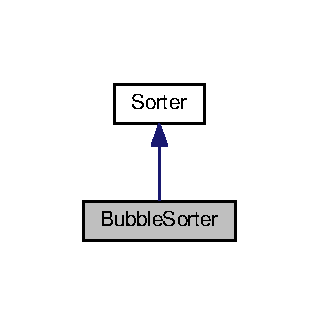
\includegraphics[width=153pt]{class_bubble_sorter__inherit__graph}
\end{center}
\end{figure}


Collaboration diagram for Bubble\+Sorter\+:
\nopagebreak
\begin{figure}[H]
\begin{center}
\leavevmode
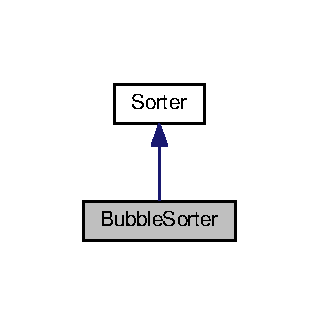
\includegraphics[width=153pt]{class_bubble_sorter__coll__graph}
\end{center}
\end{figure}
\subsection*{Public Member Functions}
\begin{DoxyCompactItemize}
\item 
\hyperlink{class_bubble_sorter_a1f4d62f7f9c513a7d3e08966b0a0670c}{Bubble\+Sorter} ()
\item 
void \hyperlink{class_bubble_sorter_ab430d94d65daffbe7ccc9e747e05b653}{sort\+In\+Place} (int $\ast$arr, int len)
\end{DoxyCompactItemize}
\subsection*{Additional Inherited Members}


\subsection{Detailed Description}
\hyperlink{class_bubble_sorter}{Bubble\+Sorter} class. 

\subsection{Constructor \& Destructor Documentation}
\index{Bubble\+Sorter@{Bubble\+Sorter}!Bubble\+Sorter@{Bubble\+Sorter}}
\index{Bubble\+Sorter@{Bubble\+Sorter}!Bubble\+Sorter@{Bubble\+Sorter}}
\subsubsection[{\texorpdfstring{Bubble\+Sorter()}{BubbleSorter()}}]{\setlength{\rightskip}{0pt plus 5cm}Bubble\+Sorter\+::\+Bubble\+Sorter (
\begin{DoxyParamCaption}
{}
\end{DoxyParamCaption}
)}\hypertarget{class_bubble_sorter_a1f4d62f7f9c513a7d3e08966b0a0670c}{}\label{class_bubble_sorter_a1f4d62f7f9c513a7d3e08966b0a0670c}
Default constructor for Sorters.

Constructs with name\+: \char`\"{}\+Bubble Sorter\char`\"{} 

\subsection{Member Function Documentation}
\index{Bubble\+Sorter@{Bubble\+Sorter}!sort\+In\+Place@{sort\+In\+Place}}
\index{sort\+In\+Place@{sort\+In\+Place}!Bubble\+Sorter@{Bubble\+Sorter}}
\subsubsection[{\texorpdfstring{sort\+In\+Place(int $\ast$arr, int len)}{sortInPlace(int *arr, int len)}}]{\setlength{\rightskip}{0pt plus 5cm}void Bubble\+Sorter\+::sort\+In\+Place (
\begin{DoxyParamCaption}
\item[{int $\ast$}]{arr, }
\item[{int}]{len}
\end{DoxyParamCaption}
)\hspace{0.3cm}{\ttfamily [virtual]}}\hypertarget{class_bubble_sorter_ab430d94d65daffbe7ccc9e747e05b653}{}\label{class_bubble_sorter_ab430d94d65daffbe7ccc9e747e05b653}
Sorts an array in place.

Uses the bubble sort algorithm. 

Implements \hyperlink{class_sorter_a946276dc986c9f017e84986c74e7cf18}{Sorter}.



The documentation for this class was generated from the following files\+:\begin{DoxyCompactItemize}
\item 
\hyperlink{_bubble_sorter_8h}{Bubble\+Sorter.\+h}\item 
\hyperlink{_bubble_sorter_8cpp}{Bubble\+Sorter.\+cpp}\end{DoxyCompactItemize}

\hypertarget{class_counting_sorter}{}\section{Counting\+Sorter Class Reference}
\label{class_counting_sorter}\index{Counting\+Sorter@{Counting\+Sorter}}


\hyperlink{class_counting_sorter}{Counting\+Sorter} class.  




{\ttfamily \#include $<$Counting\+Sorter.\+h$>$}



Inheritance diagram for Counting\+Sorter\+:\nopagebreak
\begin{figure}[H]
\begin{center}
\leavevmode
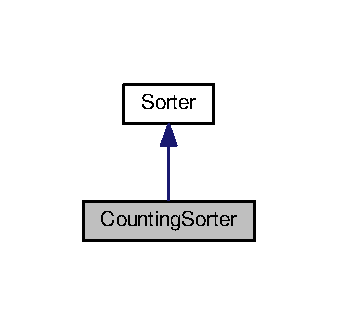
\includegraphics[width=162pt]{class_counting_sorter__inherit__graph}
\end{center}
\end{figure}


Collaboration diagram for Counting\+Sorter\+:\nopagebreak
\begin{figure}[H]
\begin{center}
\leavevmode
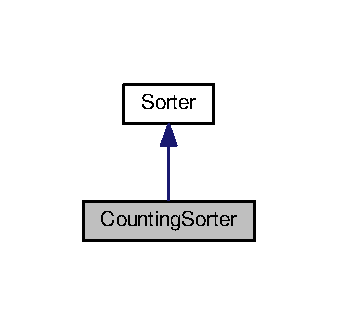
\includegraphics[width=162pt]{class_counting_sorter__coll__graph}
\end{center}
\end{figure}
\subsection*{Public Member Functions}
\begin{DoxyCompactItemize}
\item 
\hyperlink{class_counting_sorter_ad59c68b3b3190319c49a595b1cba86b7}{Counting\+Sorter} ()
\item 
void \hyperlink{class_counting_sorter_adcfc7504df3cd6e0f398a3f064bc01bc}{sort\+In\+Place} (int $\ast$arr, int len)
\end{DoxyCompactItemize}
\subsection*{Additional Inherited Members}


\subsection{Detailed Description}
\hyperlink{class_counting_sorter}{Counting\+Sorter} class. 

\subsection{Constructor \& Destructor Documentation}
\index{Counting\+Sorter@{Counting\+Sorter}!Counting\+Sorter@{Counting\+Sorter}}
\index{Counting\+Sorter@{Counting\+Sorter}!Counting\+Sorter@{Counting\+Sorter}}
\subsubsection[{\texorpdfstring{Counting\+Sorter()}{CountingSorter()}}]{\setlength{\rightskip}{0pt plus 5cm}Counting\+Sorter\+::\+Counting\+Sorter (
\begin{DoxyParamCaption}
{}
\end{DoxyParamCaption}
)}\hypertarget{class_counting_sorter_ad59c68b3b3190319c49a595b1cba86b7}{}\label{class_counting_sorter_ad59c68b3b3190319c49a595b1cba86b7}


\subsection{Member Function Documentation}
\index{Counting\+Sorter@{Counting\+Sorter}!sort\+In\+Place@{sort\+In\+Place}}
\index{sort\+In\+Place@{sort\+In\+Place}!Counting\+Sorter@{Counting\+Sorter}}
\subsubsection[{\texorpdfstring{sort\+In\+Place(int $\ast$arr, int len)}{sortInPlace(int *arr, int len)}}]{\setlength{\rightskip}{0pt plus 5cm}void Counting\+Sorter\+::sort\+In\+Place (
\begin{DoxyParamCaption}
\item[{int $\ast$}]{arr, }
\item[{int}]{len}
\end{DoxyParamCaption}
)\hspace{0.3cm}{\ttfamily [virtual]}}\hypertarget{class_counting_sorter_adcfc7504df3cd6e0f398a3f064bc01bc}{}\label{class_counting_sorter_adcfc7504df3cd6e0f398a3f064bc01bc}
Sorts an array in place.

Uses the counting sort algorithm. 

Implements \hyperlink{class_sorter_a946276dc986c9f017e84986c74e7cf18}{Sorter}.



The documentation for this class was generated from the following files\+:\begin{DoxyCompactItemize}
\item 
\hyperlink{_counting_sorter_8h}{Counting\+Sorter.\+h}\item 
\hyperlink{_counting_sorter_8cpp}{Counting\+Sorter.\+cpp}\end{DoxyCompactItemize}

\hypertarget{class_merge_sorter}{}\section{Merge\+Sorter Class Reference}
\label{class_merge_sorter}\index{Merge\+Sorter@{Merge\+Sorter}}


\hyperlink{class_merge_sorter}{Merge\+Sorter} class.  




{\ttfamily \#include $<$Merge\+Sorter.\+h$>$}



Inheritance diagram for Merge\+Sorter\+:\nopagebreak
\begin{figure}[H]
\begin{center}
\leavevmode
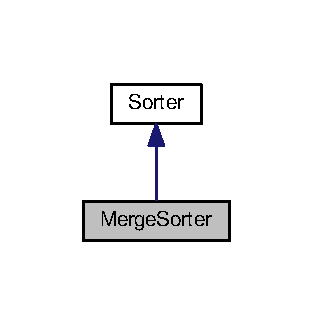
\includegraphics[width=150pt]{class_merge_sorter__inherit__graph}
\end{center}
\end{figure}


Collaboration diagram for Merge\+Sorter\+:\nopagebreak
\begin{figure}[H]
\begin{center}
\leavevmode
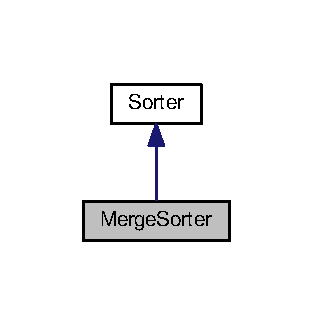
\includegraphics[width=150pt]{class_merge_sorter__coll__graph}
\end{center}
\end{figure}
\subsection*{Public Member Functions}
\begin{DoxyCompactItemize}
\item 
\hyperlink{class_merge_sorter_a6a1d4829efdea1e94f9ed2f61d32022c}{Merge\+Sorter} ()
\item 
void \hyperlink{class_merge_sorter_a1137eeb25786449a1363bac71f81014d}{sort\+In\+Place} (int $\ast$arr, int len)
\end{DoxyCompactItemize}
\subsection*{Private Member Functions}
\begin{DoxyCompactItemize}
\item 
void \hyperlink{class_merge_sorter_aeb7003d6bbbe8963f65df7d6e5b11d15}{merge\+Parts} (int $\ast$part1, int len1, int $\ast$part2, int len2, int $\ast$dest)
\begin{DoxyCompactList}\small\item\em Merge two arrays in the right way. \end{DoxyCompactList}\item 
void \hyperlink{class_merge_sorter_a13bb5ca817e9159b33324d2db33d7d61}{sort\+Recursive} (int $\ast$arr, int len)
\begin{DoxyCompactList}\small\item\em The recursive layer for merge sort. \end{DoxyCompactList}\end{DoxyCompactItemize}
\subsection*{Additional Inherited Members}


\subsection{Detailed Description}
\hyperlink{class_merge_sorter}{Merge\+Sorter} class. 

\subsection{Constructor \& Destructor Documentation}
\index{Merge\+Sorter@{Merge\+Sorter}!Merge\+Sorter@{Merge\+Sorter}}
\index{Merge\+Sorter@{Merge\+Sorter}!Merge\+Sorter@{Merge\+Sorter}}
\subsubsection[{\texorpdfstring{Merge\+Sorter()}{MergeSorter()}}]{\setlength{\rightskip}{0pt plus 5cm}Merge\+Sorter\+::\+Merge\+Sorter (
\begin{DoxyParamCaption}
{}
\end{DoxyParamCaption}
)}\hypertarget{class_merge_sorter_a6a1d4829efdea1e94f9ed2f61d32022c}{}\label{class_merge_sorter_a6a1d4829efdea1e94f9ed2f61d32022c}
Default constructor for Sorters.

Constructs with name\+: \char`\"{}\+Merge Sorter\char`\"{} 

\subsection{Member Function Documentation}
\index{Merge\+Sorter@{Merge\+Sorter}!merge\+Parts@{merge\+Parts}}
\index{merge\+Parts@{merge\+Parts}!Merge\+Sorter@{Merge\+Sorter}}
\subsubsection[{\texorpdfstring{merge\+Parts(int $\ast$part1, int len1, int $\ast$part2, int len2, int $\ast$dest)}{mergeParts(int *part1, int len1, int *part2, int len2, int *dest)}}]{\setlength{\rightskip}{0pt plus 5cm}void Merge\+Sorter\+::merge\+Parts (
\begin{DoxyParamCaption}
\item[{int $\ast$}]{part1, }
\item[{int}]{len1, }
\item[{int $\ast$}]{part2, }
\item[{int}]{len2, }
\item[{int $\ast$}]{dest}
\end{DoxyParamCaption}
)\hspace{0.3cm}{\ttfamily [private]}}\hypertarget{class_merge_sorter_aeb7003d6bbbe8963f65df7d6e5b11d15}{}\label{class_merge_sorter_aeb7003d6bbbe8963f65df7d6e5b11d15}


Merge two arrays in the right way. 


\begin{DoxyParams}{Parameters}
{\em part1} & The first part to merge. \\
\hline
{\em len1} & The length of the first part. \\
\hline
{\em part2} & The second part to merge. \\
\hline
{\em len2} & The length of the second part. \\
\hline
{\em dest} & The merge destination. \\
\hline
\end{DoxyParams}
\begin{DoxyPrecond}{Precondition}
The length of dest $>$= len1+len2 
\end{DoxyPrecond}
\index{Merge\+Sorter@{Merge\+Sorter}!sort\+In\+Place@{sort\+In\+Place}}
\index{sort\+In\+Place@{sort\+In\+Place}!Merge\+Sorter@{Merge\+Sorter}}
\subsubsection[{\texorpdfstring{sort\+In\+Place(int $\ast$arr, int len)}{sortInPlace(int *arr, int len)}}]{\setlength{\rightskip}{0pt plus 5cm}void Merge\+Sorter\+::sort\+In\+Place (
\begin{DoxyParamCaption}
\item[{int $\ast$}]{arr, }
\item[{int}]{len}
\end{DoxyParamCaption}
)\hspace{0.3cm}{\ttfamily [virtual]}}\hypertarget{class_merge_sorter_a1137eeb25786449a1363bac71f81014d}{}\label{class_merge_sorter_a1137eeb25786449a1363bac71f81014d}
Sorts an array in place.

Uses the merge sort algorithm. 

Implements \hyperlink{class_sorter_a946276dc986c9f017e84986c74e7cf18}{Sorter}.

\index{Merge\+Sorter@{Merge\+Sorter}!sort\+Recursive@{sort\+Recursive}}
\index{sort\+Recursive@{sort\+Recursive}!Merge\+Sorter@{Merge\+Sorter}}
\subsubsection[{\texorpdfstring{sort\+Recursive(int $\ast$arr, int len)}{sortRecursive(int *arr, int len)}}]{\setlength{\rightskip}{0pt plus 5cm}void Merge\+Sorter\+::sort\+Recursive (
\begin{DoxyParamCaption}
\item[{int $\ast$}]{arr, }
\item[{int}]{len}
\end{DoxyParamCaption}
)\hspace{0.3cm}{\ttfamily [private]}}\hypertarget{class_merge_sorter_a13bb5ca817e9159b33324d2db33d7d61}{}\label{class_merge_sorter_a13bb5ca817e9159b33324d2db33d7d61}


The recursive layer for merge sort. 


\begin{DoxyParams}{Parameters}
{\em arr} & The array to sort. \\
\hline
{\em len} & The length of the array to sort \\
\hline
\end{DoxyParams}


The documentation for this class was generated from the following files\+:\begin{DoxyCompactItemize}
\item 
\hyperlink{_merge_sorter_8h}{Merge\+Sorter.\+h}\item 
\hyperlink{_merge_sorter_8cpp}{Merge\+Sorter.\+cpp}\end{DoxyCompactItemize}

\hypertarget{class_sorter}{}\section{Sorter Class Reference}
\label{class_sorter}\index{Sorter@{Sorter}}


Base class for \hyperlink{class_sorter}{Sorter} classes, which sort int data.  




{\ttfamily \#include $<$Sorter.\+h$>$}



Inheritance diagram for Sorter\+:\nopagebreak
\begin{figure}[H]
\begin{center}
\leavevmode
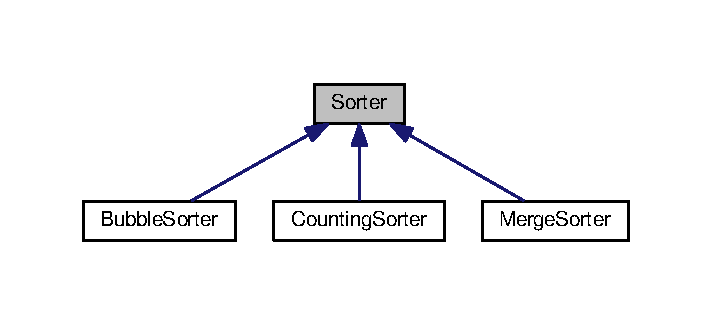
\includegraphics[width=342pt]{class_sorter__inherit__graph}
\end{center}
\end{figure}
\subsection*{Public Member Functions}
\begin{DoxyCompactItemize}
\item 
\hyperlink{class_sorter_a0b2a0bc2bae60db1115788f49f988859}{Sorter} ()
\begin{DoxyCompactList}\small\item\em Default constructor for Sorters. \end{DoxyCompactList}\item 
virtual void \hyperlink{class_sorter_a946276dc986c9f017e84986c74e7cf18}{sort\+In\+Place} (int $\ast$arr, int len)=0
\begin{DoxyCompactList}\small\item\em Sorts an array in place. \end{DoxyCompactList}\item 
\hyperlink{struct_sort_stats}{Sort\+Stats} \hyperlink{class_sorter_af864ce19b5f14a410ab55c1af6b4e3a5}{get\+Stats} ()
\begin{DoxyCompactList}\small\item\em Returns statistics on all sorts performed. \end{DoxyCompactList}\item 
void \hyperlink{class_sorter_a085f06b5b3200a426c05fab3eca30dfe}{reset\+Stats} ()
\begin{DoxyCompactList}\small\item\em Resets the stats. \end{DoxyCompactList}\item 
std\+::string \hyperlink{class_sorter_aa7596dcc44254c88e2544708adff0de0}{get\+Name} ()
\begin{DoxyCompactList}\small\item\em Gets the name of this sorter. \end{DoxyCompactList}\end{DoxyCompactItemize}
\subsection*{Protected Member Functions}
\begin{DoxyCompactItemize}
\item 
void \hyperlink{class_sorter_a706bb59cd4957fe8e7b2eb46f1a09092}{start\+Timer} ()
\begin{DoxyCompactList}\small\item\em Starts timing the algorithm. \end{DoxyCompactList}\item 
void \hyperlink{class_sorter_a2aff740358afb37276666168cf059f62}{stop\+Timer} ()
\begin{DoxyCompactList}\small\item\em Stops timing the algorithm and adds the elapsed time to tot\+Time. \end{DoxyCompactList}\end{DoxyCompactItemize}
\subsection*{Protected Attributes}
\begin{DoxyCompactItemize}
\item 
int \hyperlink{class_sorter_a582afc82309a3bf0e5567814b6d61079}{sorts\+Run}
\item 
long \hyperlink{class_sorter_afd76a62edf3a0f6ed7a2eee28335e42f}{tot\+Time}
\item 
long \hyperlink{class_sorter_a28ba087dad25b8c837c1211d8d2cb8f4}{tot\+Num\+Comparisons}
\item 
long \hyperlink{class_sorter_a2fcaa452c03ec3429bedd8de1421e678}{tot\+Num\+Swaps}
\item 
std\+::string \hyperlink{class_sorter_ae86338aba4991d9a1376400733579f4f}{name}
\item 
std\+::chrono\+::time\+\_\+point$<$ std\+::chrono\+::high\+\_\+resolution\+\_\+clock $>$ \hyperlink{class_sorter_a022bf8dfe39ec74d4761fe9c9b0f5915}{tmr\+Start}
\end{DoxyCompactItemize}


\subsection{Detailed Description}
Base class for \hyperlink{class_sorter}{Sorter} classes, which sort int data. 

\hyperlink{class_sorter}{Sorter} classes record various statistics on the sort. 

\subsection{Constructor \& Destructor Documentation}
\index{Sorter@{Sorter}!Sorter@{Sorter}}
\index{Sorter@{Sorter}!Sorter@{Sorter}}
\subsubsection[{\texorpdfstring{Sorter()}{Sorter()}}]{\setlength{\rightskip}{0pt plus 5cm}Sorter\+::\+Sorter (
\begin{DoxyParamCaption}
{}
\end{DoxyParamCaption}
)}\hypertarget{class_sorter_a0b2a0bc2bae60db1115788f49f988859}{}\label{class_sorter_a0b2a0bc2bae60db1115788f49f988859}


Default constructor for Sorters. 

Constructs with name\+: \char`\"{}\+Base Sorter\char`\"{} 

\subsection{Member Function Documentation}
\index{Sorter@{Sorter}!get\+Name@{get\+Name}}
\index{get\+Name@{get\+Name}!Sorter@{Sorter}}
\subsubsection[{\texorpdfstring{get\+Name()}{getName()}}]{\setlength{\rightskip}{0pt plus 5cm}std\+::string Sorter\+::get\+Name (
\begin{DoxyParamCaption}
{}
\end{DoxyParamCaption}
)}\hypertarget{class_sorter_aa7596dcc44254c88e2544708adff0de0}{}\label{class_sorter_aa7596dcc44254c88e2544708adff0de0}


Gets the name of this sorter. 

\begin{DoxyReturn}{Returns}
The name of this sorter. 
\end{DoxyReturn}
\index{Sorter@{Sorter}!get\+Stats@{get\+Stats}}
\index{get\+Stats@{get\+Stats}!Sorter@{Sorter}}
\subsubsection[{\texorpdfstring{get\+Stats()}{getStats()}}]{\setlength{\rightskip}{0pt plus 5cm}{\bf Sort\+Stats} Sorter\+::get\+Stats (
\begin{DoxyParamCaption}
{}
\end{DoxyParamCaption}
)}\hypertarget{class_sorter_af864ce19b5f14a410ab55c1af6b4e3a5}{}\label{class_sorter_af864ce19b5f14a410ab55c1af6b4e3a5}


Returns statistics on all sorts performed. 

\begin{DoxyReturn}{Returns}
A filled \hyperlink{struct_sort_stats}{Sort\+Stats} instance. 
\end{DoxyReturn}
\index{Sorter@{Sorter}!reset\+Stats@{reset\+Stats}}
\index{reset\+Stats@{reset\+Stats}!Sorter@{Sorter}}
\subsubsection[{\texorpdfstring{reset\+Stats()}{resetStats()}}]{\setlength{\rightskip}{0pt plus 5cm}void Sorter\+::reset\+Stats (
\begin{DoxyParamCaption}
{}
\end{DoxyParamCaption}
)}\hypertarget{class_sorter_a085f06b5b3200a426c05fab3eca30dfe}{}\label{class_sorter_a085f06b5b3200a426c05fab3eca30dfe}


Resets the stats. 

\index{Sorter@{Sorter}!sort\+In\+Place@{sort\+In\+Place}}
\index{sort\+In\+Place@{sort\+In\+Place}!Sorter@{Sorter}}
\subsubsection[{\texorpdfstring{sort\+In\+Place(int $\ast$arr, int len)=0}{sortInPlace(int *arr, int len)=0}}]{\setlength{\rightskip}{0pt plus 5cm}virtual void Sorter\+::sort\+In\+Place (
\begin{DoxyParamCaption}
\item[{int $\ast$}]{arr, }
\item[{int}]{len}
\end{DoxyParamCaption}
)\hspace{0.3cm}{\ttfamily [pure virtual]}}\hypertarget{class_sorter_a946276dc986c9f017e84986c74e7cf18}{}\label{class_sorter_a946276dc986c9f017e84986c74e7cf18}


Sorts an array in place. 


\begin{DoxyParams}{Parameters}
{\em arr} & The array to sort. \\
\hline
{\em len} & The length of the array to sort. \\
\hline
\end{DoxyParams}
\begin{DoxyPrecond}{Precondition}
The given array is at least len long.
\end{DoxyPrecond}
Algorithm is abstracted. 

Implemented in \hyperlink{class_merge_sorter_a1137eeb25786449a1363bac71f81014d}{Merge\+Sorter}, \hyperlink{class_bubble_sorter_ab430d94d65daffbe7ccc9e747e05b653}{Bubble\+Sorter}, and \hyperlink{class_counting_sorter_adcfc7504df3cd6e0f398a3f064bc01bc}{Counting\+Sorter}.

\index{Sorter@{Sorter}!start\+Timer@{start\+Timer}}
\index{start\+Timer@{start\+Timer}!Sorter@{Sorter}}
\subsubsection[{\texorpdfstring{start\+Timer()}{startTimer()}}]{\setlength{\rightskip}{0pt plus 5cm}void Sorter\+::start\+Timer (
\begin{DoxyParamCaption}
{}
\end{DoxyParamCaption}
)\hspace{0.3cm}{\ttfamily [protected]}}\hypertarget{class_sorter_a706bb59cd4957fe8e7b2eb46f1a09092}{}\label{class_sorter_a706bb59cd4957fe8e7b2eb46f1a09092}


Starts timing the algorithm. 

\begin{DoxyPrecond}{Precondition}
The timer is stopped. 
\end{DoxyPrecond}
\index{Sorter@{Sorter}!stop\+Timer@{stop\+Timer}}
\index{stop\+Timer@{stop\+Timer}!Sorter@{Sorter}}
\subsubsection[{\texorpdfstring{stop\+Timer()}{stopTimer()}}]{\setlength{\rightskip}{0pt plus 5cm}void Sorter\+::stop\+Timer (
\begin{DoxyParamCaption}
{}
\end{DoxyParamCaption}
)\hspace{0.3cm}{\ttfamily [protected]}}\hypertarget{class_sorter_a2aff740358afb37276666168cf059f62}{}\label{class_sorter_a2aff740358afb37276666168cf059f62}


Stops timing the algorithm and adds the elapsed time to tot\+Time. 

\begin{DoxyPrecond}{Precondition}
The timer has been started. 
\end{DoxyPrecond}


\subsection{Member Data Documentation}
\index{Sorter@{Sorter}!name@{name}}
\index{name@{name}!Sorter@{Sorter}}
\subsubsection[{\texorpdfstring{name}{name}}]{\setlength{\rightskip}{0pt plus 5cm}std\+::string Sorter\+::name\hspace{0.3cm}{\ttfamily [protected]}}\hypertarget{class_sorter_ae86338aba4991d9a1376400733579f4f}{}\label{class_sorter_ae86338aba4991d9a1376400733579f4f}
\index{Sorter@{Sorter}!sorts\+Run@{sorts\+Run}}
\index{sorts\+Run@{sorts\+Run}!Sorter@{Sorter}}
\subsubsection[{\texorpdfstring{sorts\+Run}{sortsRun}}]{\setlength{\rightskip}{0pt plus 5cm}int Sorter\+::sorts\+Run\hspace{0.3cm}{\ttfamily [protected]}}\hypertarget{class_sorter_a582afc82309a3bf0e5567814b6d61079}{}\label{class_sorter_a582afc82309a3bf0e5567814b6d61079}
\index{Sorter@{Sorter}!tmr\+Start@{tmr\+Start}}
\index{tmr\+Start@{tmr\+Start}!Sorter@{Sorter}}
\subsubsection[{\texorpdfstring{tmr\+Start}{tmrStart}}]{\setlength{\rightskip}{0pt plus 5cm}std\+::chrono\+::time\+\_\+point$<$std\+::chrono\+::high\+\_\+resolution\+\_\+clock$>$ Sorter\+::tmr\+Start\hspace{0.3cm}{\ttfamily [protected]}}\hypertarget{class_sorter_a022bf8dfe39ec74d4761fe9c9b0f5915}{}\label{class_sorter_a022bf8dfe39ec74d4761fe9c9b0f5915}
\index{Sorter@{Sorter}!tot\+Num\+Comparisons@{tot\+Num\+Comparisons}}
\index{tot\+Num\+Comparisons@{tot\+Num\+Comparisons}!Sorter@{Sorter}}
\subsubsection[{\texorpdfstring{tot\+Num\+Comparisons}{totNumComparisons}}]{\setlength{\rightskip}{0pt plus 5cm}long Sorter\+::tot\+Num\+Comparisons\hspace{0.3cm}{\ttfamily [protected]}}\hypertarget{class_sorter_a28ba087dad25b8c837c1211d8d2cb8f4}{}\label{class_sorter_a28ba087dad25b8c837c1211d8d2cb8f4}
\index{Sorter@{Sorter}!tot\+Num\+Swaps@{tot\+Num\+Swaps}}
\index{tot\+Num\+Swaps@{tot\+Num\+Swaps}!Sorter@{Sorter}}
\subsubsection[{\texorpdfstring{tot\+Num\+Swaps}{totNumSwaps}}]{\setlength{\rightskip}{0pt plus 5cm}long Sorter\+::tot\+Num\+Swaps\hspace{0.3cm}{\ttfamily [protected]}}\hypertarget{class_sorter_a2fcaa452c03ec3429bedd8de1421e678}{}\label{class_sorter_a2fcaa452c03ec3429bedd8de1421e678}
\index{Sorter@{Sorter}!tot\+Time@{tot\+Time}}
\index{tot\+Time@{tot\+Time}!Sorter@{Sorter}}
\subsubsection[{\texorpdfstring{tot\+Time}{totTime}}]{\setlength{\rightskip}{0pt plus 5cm}long Sorter\+::tot\+Time\hspace{0.3cm}{\ttfamily [protected]}}\hypertarget{class_sorter_afd76a62edf3a0f6ed7a2eee28335e42f}{}\label{class_sorter_afd76a62edf3a0f6ed7a2eee28335e42f}


The documentation for this class was generated from the following files\+:\begin{DoxyCompactItemize}
\item 
\hyperlink{_sorter_8h}{Sorter.\+h}\item 
\hyperlink{_sorter_8cpp}{Sorter.\+cpp}\end{DoxyCompactItemize}

\hypertarget{struct_sort_stats}{}\section{Sort\+Stats Struct Reference}
\label{struct_sort_stats}\index{Sort\+Stats@{Sort\+Stats}}


Contains sorting statistics.  




{\ttfamily \#include $<$Sorter.\+h$>$}

\subsection*{Public Attributes}
\begin{DoxyCompactItemize}
\item 
float \hyperlink{struct_sort_stats_a11a7890287500982a8d08d5ea9da2bbb}{avg\+C\+P\+U\+Time}
\item 
float \hyperlink{struct_sort_stats_a7566917dde7a1cfefbe2775c858413c1}{avg\+Num\+Comparisons}
\item 
float \hyperlink{struct_sort_stats_a0ce1570721d9b686f9fa0adb164689df}{avg\+Num\+Swaps}
\end{DoxyCompactItemize}


\subsection{Detailed Description}
Contains sorting statistics. 

\subsection{Member Data Documentation}
\index{Sort\+Stats@{Sort\+Stats}!avg\+C\+P\+U\+Time@{avg\+C\+P\+U\+Time}}
\index{avg\+C\+P\+U\+Time@{avg\+C\+P\+U\+Time}!Sort\+Stats@{Sort\+Stats}}
\subsubsection[{\texorpdfstring{avg\+C\+P\+U\+Time}{avgCPUTime}}]{\setlength{\rightskip}{0pt plus 5cm}float Sort\+Stats\+::avg\+C\+P\+U\+Time}\hypertarget{struct_sort_stats_a11a7890287500982a8d08d5ea9da2bbb}{}\label{struct_sort_stats_a11a7890287500982a8d08d5ea9da2bbb}
\index{Sort\+Stats@{Sort\+Stats}!avg\+Num\+Comparisons@{avg\+Num\+Comparisons}}
\index{avg\+Num\+Comparisons@{avg\+Num\+Comparisons}!Sort\+Stats@{Sort\+Stats}}
\subsubsection[{\texorpdfstring{avg\+Num\+Comparisons}{avgNumComparisons}}]{\setlength{\rightskip}{0pt plus 5cm}float Sort\+Stats\+::avg\+Num\+Comparisons}\hypertarget{struct_sort_stats_a7566917dde7a1cfefbe2775c858413c1}{}\label{struct_sort_stats_a7566917dde7a1cfefbe2775c858413c1}
\index{Sort\+Stats@{Sort\+Stats}!avg\+Num\+Swaps@{avg\+Num\+Swaps}}
\index{avg\+Num\+Swaps@{avg\+Num\+Swaps}!Sort\+Stats@{Sort\+Stats}}
\subsubsection[{\texorpdfstring{avg\+Num\+Swaps}{avgNumSwaps}}]{\setlength{\rightskip}{0pt plus 5cm}float Sort\+Stats\+::avg\+Num\+Swaps}\hypertarget{struct_sort_stats_a0ce1570721d9b686f9fa0adb164689df}{}\label{struct_sort_stats_a0ce1570721d9b686f9fa0adb164689df}


The documentation for this struct was generated from the following file\+:\begin{DoxyCompactItemize}
\item 
\hyperlink{_sorter_8h}{Sorter.\+h}\end{DoxyCompactItemize}

\chapter{File Documentation}
\hypertarget{_bubble_sorter_8cpp}{}\section{Bubble\+Sorter.\+cpp File Reference}
\label{_bubble_sorter_8cpp}\index{Bubble\+Sorter.\+cpp@{Bubble\+Sorter.\+cpp}}


Implementation file for the \hyperlink{class_bubble_sorter}{Bubble\+Sorter} class.  


{\ttfamily \#include \char`\"{}Bubble\+Sorter.\+h\char`\"{}}\\*
{\ttfamily \#include $<$utility$>$}\\*
{\ttfamily \#include $<$ctime$>$}\\*
Include dependency graph for Bubble\+Sorter.\+cpp\+:
\nopagebreak
\begin{figure}[H]
\begin{center}
\leavevmode
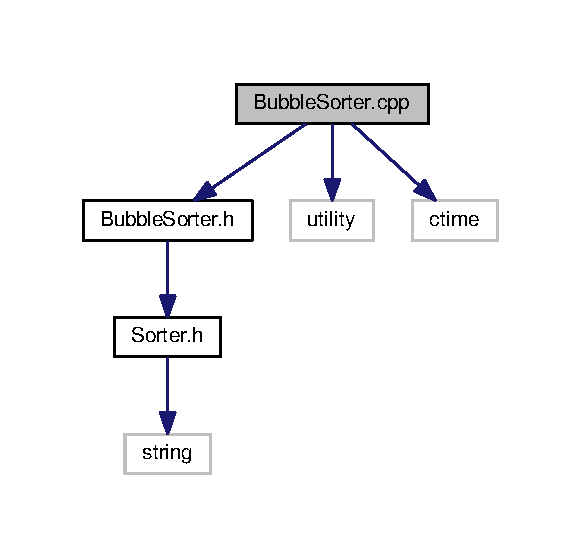
\includegraphics[width=279pt]{_bubble_sorter_8cpp__incl}
\end{center}
\end{figure}


\subsection{Detailed Description}
Implementation file for the \hyperlink{class_bubble_sorter}{Bubble\+Sorter} class. 

\begin{DoxyAuthor}{Author}
Matthew Bauer 
\end{DoxyAuthor}

\hypertarget{_bubble_sorter_8h}{}\section{Bubble\+Sorter.\+h File Reference}
\label{_bubble_sorter_8h}\index{Bubble\+Sorter.\+h@{Bubble\+Sorter.\+h}}


Delcaration file for the \hyperlink{class_bubble_sorter}{Bubble\+Sorter} class.  


{\ttfamily \#include \char`\"{}Sorter.\+h\char`\"{}}\\*
Include dependency graph for Bubble\+Sorter.\+h\+:
\nopagebreak
\begin{figure}[H]
\begin{center}
\leavevmode
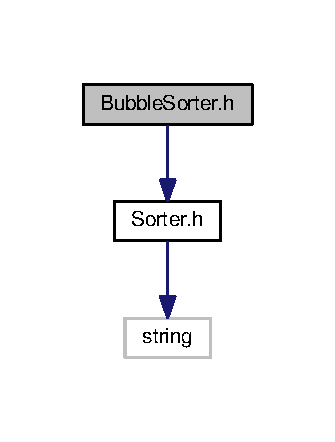
\includegraphics[width=186pt]{_bubble_sorter_8h__incl}
\end{center}
\end{figure}
This graph shows which files directly or indirectly include this file\+:\nopagebreak
\begin{figure}[H]
\begin{center}
\leavevmode
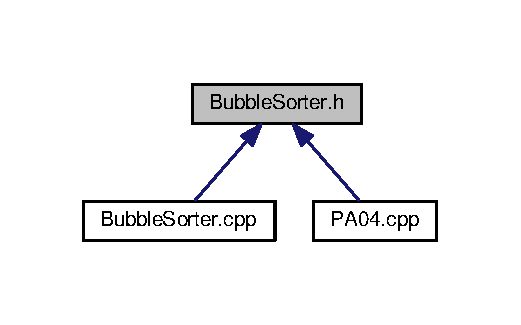
\includegraphics[width=250pt]{_bubble_sorter_8h__dep__incl}
\end{center}
\end{figure}
\subsection*{Classes}
\begin{DoxyCompactItemize}
\item 
class \hyperlink{class_bubble_sorter}{Bubble\+Sorter}
\begin{DoxyCompactList}\small\item\em \hyperlink{class_bubble_sorter}{Bubble\+Sorter} class. \end{DoxyCompactList}\end{DoxyCompactItemize}


\subsection{Detailed Description}
Delcaration file for the \hyperlink{class_bubble_sorter}{Bubble\+Sorter} class. 

\begin{DoxyAuthor}{Author}
Matthew Bauer 
\end{DoxyAuthor}

\hypertarget{_counting_sorter_8cpp}{}\section{Counting\+Sorter.\+cpp File Reference}
\label{_counting_sorter_8cpp}\index{Counting\+Sorter.\+cpp@{Counting\+Sorter.\+cpp}}


Implementation file for the \hyperlink{class_counting_sorter}{Counting\+Sorter} class.  


{\ttfamily \#include \char`\"{}Counting\+Sorter.\+h\char`\"{}}\\*
{\ttfamily \#include $<$ctime$>$}\\*
{\ttfamily \#include $<$string.\+h$>$}\\*
Include dependency graph for Counting\+Sorter.\+cpp\+:
\nopagebreak
\begin{figure}[H]
\begin{center}
\leavevmode
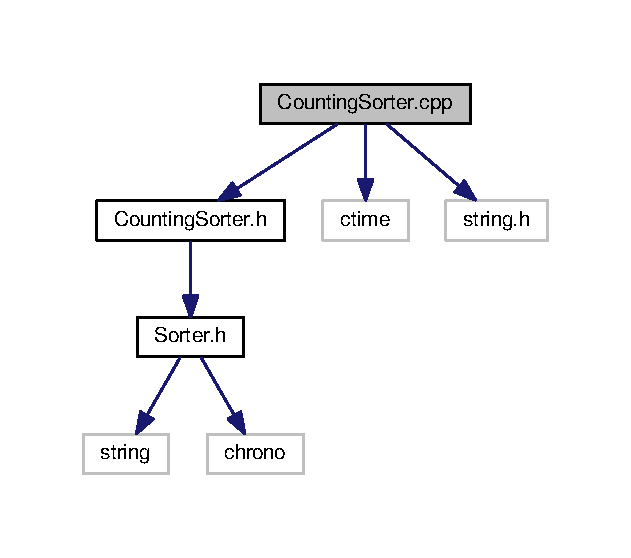
\includegraphics[width=303pt]{_counting_sorter_8cpp__incl}
\end{center}
\end{figure}


\subsection{Detailed Description}
Implementation file for the \hyperlink{class_counting_sorter}{Counting\+Sorter} class. 

\begin{DoxyAuthor}{Author}
Matthew Bauer 
\end{DoxyAuthor}

\hypertarget{_counting_sorter_8h}{}\section{Counting\+Sorter.\+h File Reference}
\label{_counting_sorter_8h}\index{Counting\+Sorter.\+h@{Counting\+Sorter.\+h}}


Declaration file for the \hyperlink{class_counting_sorter}{Counting\+Sorter} class.  


{\ttfamily \#include \char`\"{}Sorter.\+h\char`\"{}}\\*
Include dependency graph for Counting\+Sorter.\+h\+:
\nopagebreak
\begin{figure}[H]
\begin{center}
\leavevmode
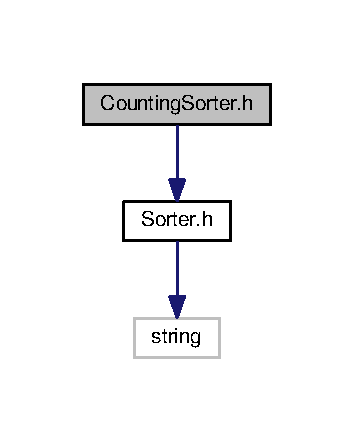
\includegraphics[width=170pt]{_counting_sorter_8h__incl}
\end{center}
\end{figure}
This graph shows which files directly or indirectly include this file\+:
\nopagebreak
\begin{figure}[H]
\begin{center}
\leavevmode
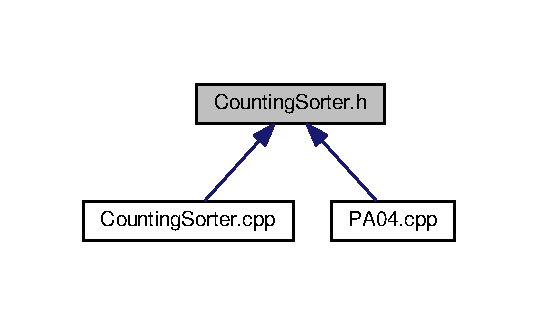
\includegraphics[width=258pt]{_counting_sorter_8h__dep__incl}
\end{center}
\end{figure}
\subsection*{Classes}
\begin{DoxyCompactItemize}
\item 
class \hyperlink{class_counting_sorter}{Counting\+Sorter}
\begin{DoxyCompactList}\small\item\em \hyperlink{class_counting_sorter}{Counting\+Sorter} class. \end{DoxyCompactList}\end{DoxyCompactItemize}


\subsection{Detailed Description}
Declaration file for the \hyperlink{class_counting_sorter}{Counting\+Sorter} class. 

\begin{DoxyAuthor}{Author}
Matthew Bauer 
\end{DoxyAuthor}

\hypertarget{_merge_sorter_8cpp}{}\section{Merge\+Sorter.\+cpp File Reference}
\label{_merge_sorter_8cpp}\index{Merge\+Sorter.\+cpp@{Merge\+Sorter.\+cpp}}


Implementation file for the \hyperlink{class_merge_sorter}{Merge\+Sorter} class.  


{\ttfamily \#include \char`\"{}Merge\+Sorter.\+h\char`\"{}}\\*
{\ttfamily \#include $<$ctime$>$}\\*
{\ttfamily \#include $<$string.\+h$>$}\\*
Include dependency graph for Merge\+Sorter.\+cpp\+:
\nopagebreak
\begin{figure}[H]
\begin{center}
\leavevmode
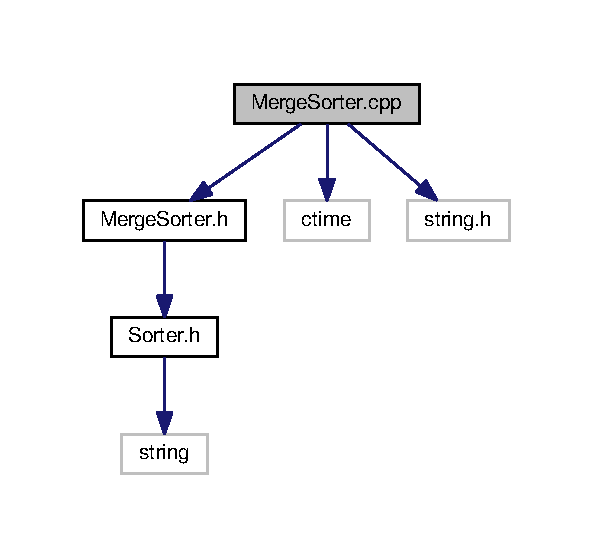
\includegraphics[width=285pt]{_merge_sorter_8cpp__incl}
\end{center}
\end{figure}


\subsection{Detailed Description}
Implementation file for the \hyperlink{class_merge_sorter}{Merge\+Sorter} class. 

\begin{DoxyAuthor}{Author}
Matthew Bauer 
\end{DoxyAuthor}

\hypertarget{_merge_sorter_8h}{}\section{Merge\+Sorter.\+h File Reference}
\label{_merge_sorter_8h}\index{Merge\+Sorter.\+h@{Merge\+Sorter.\+h}}


Declaration file for the \hyperlink{class_merge_sorter}{Merge\+Sorter} class.  


{\ttfamily \#include \char`\"{}Sorter.\+h\char`\"{}}\\*
Include dependency graph for Merge\+Sorter.\+h\+:
\nopagebreak
\begin{figure}[H]
\begin{center}
\leavevmode
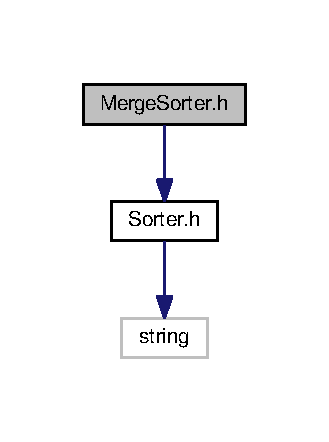
\includegraphics[width=158pt]{_merge_sorter_8h__incl}
\end{center}
\end{figure}
This graph shows which files directly or indirectly include this file\+:
\nopagebreak
\begin{figure}[H]
\begin{center}
\leavevmode
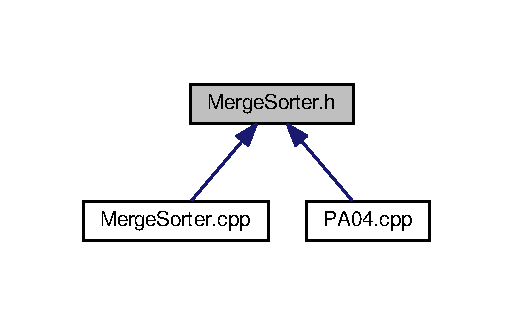
\includegraphics[width=246pt]{_merge_sorter_8h__dep__incl}
\end{center}
\end{figure}
\subsection*{Classes}
\begin{DoxyCompactItemize}
\item 
class \hyperlink{class_merge_sorter}{Merge\+Sorter}
\begin{DoxyCompactList}\small\item\em \hyperlink{class_merge_sorter}{Merge\+Sorter} class. \end{DoxyCompactList}\end{DoxyCompactItemize}


\subsection{Detailed Description}
Declaration file for the \hyperlink{class_merge_sorter}{Merge\+Sorter} class. 

\begin{DoxyAuthor}{Author}
Matthew Bauer 
\end{DoxyAuthor}

\hypertarget{_p_a04_8cpp}{}\section{P\+A04.\+cpp File Reference}
\label{_p_a04_8cpp}\index{P\+A04.\+cpp@{P\+A04.\+cpp}}


Main file for C\+S302/\+P\+A04.  


{\ttfamily \#include $<$iostream$>$}\\*
{\ttfamily \#include $<$cstdlib$>$}\\*
{\ttfamily \#include $<$ctime$>$}\\*
{\ttfamily \#include $<$vector$>$}\\*
{\ttfamily \#include $<$sstream$>$}\\*
{\ttfamily \#include $<$string.\+h$>$}\\*
{\ttfamily \#include $<$fstream$>$}\\*
{\ttfamily \#include \char`\"{}Bubble\+Sorter.\+h\char`\"{}}\\*
{\ttfamily \#include \char`\"{}Merge\+Sorter.\+h\char`\"{}}\\*
{\ttfamily \#include \char`\"{}Counting\+Sorter.\+h\char`\"{}}\\*
Include dependency graph for P\+A04.\+cpp\+:
\nopagebreak
\begin{figure}[H]
\begin{center}
\leavevmode
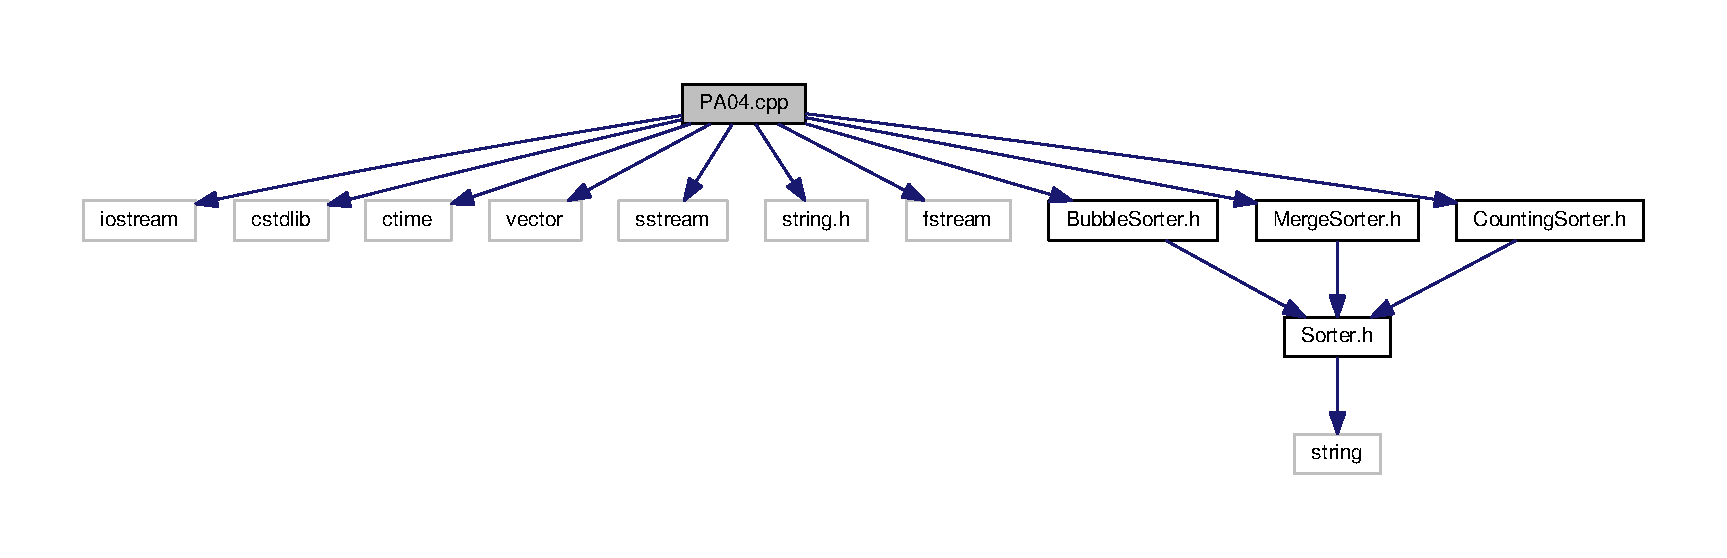
\includegraphics[width=350pt]{_p_a04_8cpp__incl}
\end{center}
\end{figure}
\subsection*{Functions}
\begin{DoxyCompactItemize}
\item 
void \hyperlink{_p_a04_8cpp_a4573cd9c09b30d379f0c47f2ec14e7b9}{fill\+Array\+Randomly} (int $\ast$arr, int num\+Ints)
\begin{DoxyCompactList}\small\item\em Fills an array with the given number of random integers with values ranging from 0 to 1000000. \end{DoxyCompactList}\item 
void \hyperlink{_p_a04_8cpp_a733045b67e1b8242db2b77c270025ff6}{fill\+Randset} (int $\ast$$\ast$\&set, int nval)
\begin{DoxyCompactList}\small\item\em Fill one randset. \end{DoxyCompactList}\item 
void \hyperlink{_p_a04_8cpp_a00f93c6504af37640753e6e7153a20ee}{generate\+Randsets} ()
\begin{DoxyCompactList}\small\item\em Fill all randsets appropriately. \end{DoxyCompactList}\item 
void \hyperlink{_p_a04_8cpp_a88fe60bfd6f33c3bd41d57c8da43a80f}{free\+One\+Randset} (int $\ast$$\ast$\&set)
\begin{DoxyCompactList}\small\item\em Free one randset. \end{DoxyCompactList}\item 
void \hyperlink{_p_a04_8cpp_a05e464736d72893d788140acf09b2d24}{free\+Randsets} ()
\begin{DoxyCompactList}\small\item\em Free the memory of all randsets. \end{DoxyCompactList}\item 
void \hyperlink{_p_a04_8cpp_a472101d67480be401c7070a1feda447e}{test\+Array} (\hyperlink{class_sorter}{Sorter} $\ast$sorter, int $\ast$arr, int len, std\+::stringstream \&sort\+Out, bool write\+Out=false)
\begin{DoxyCompactList}\small\item\em Test an array on a \hyperlink{class_sorter}{Sorter}. \end{DoxyCompactList}\item 
void \hyperlink{_p_a04_8cpp_aad638c13d38642ca2be432c4c542693a}{test\+Randset} (\hyperlink{class_sorter}{Sorter} $\ast$sorter, int $\ast$$\ast$set, int len, std\+::stringstream \&sort\+Out, std\+::stringstream \&stat\+Out)
\begin{DoxyCompactList}\small\item\em Test a randset on a \hyperlink{class_sorter}{Sorter}. \end{DoxyCompactList}\item 
void \hyperlink{_p_a04_8cpp_a54006df013b428e99d043289cfc7e292}{test\+One\+Sorter} (\hyperlink{class_sorter}{Sorter} $\ast$sorter, std\+::stringstream \&sort\+Out, std\+::stringstream \&stat\+Out)
\begin{DoxyCompactList}\small\item\em Test a \hyperlink{class_sorter}{Sorter} on various data. \end{DoxyCompactList}\item 
void \hyperlink{_p_a04_8cpp_addbc6930265a35072360c819a6e67a93}{test\+Sorters} (std\+::stringstream \&sort\+Out, std\+::stringstream \&stat\+Out)
\begin{DoxyCompactList}\small\item\em Tests all Sorters fully. \end{DoxyCompactList}\item 
int \hyperlink{_p_a04_8cpp_ae66f6b31b5ad750f1fe042a706a4e3d4}{main} ()
\begin{DoxyCompactList}\small\item\em Entry point. \end{DoxyCompactList}\end{DoxyCompactItemize}
\subsection*{Variables}
\begin{DoxyCompactItemize}
\item 
int $\ast$$\ast$ \hyperlink{_p_a04_8cpp_aed17f6d6f6eac3b72ab37430e2c0e03b}{randset\+\_\+1k}
\item 
int $\ast$$\ast$ \hyperlink{_p_a04_8cpp_aaa405254ce6444ad19c4ff8303c53c15}{randset\+\_\+10k}
\item 
int $\ast$$\ast$ \hyperlink{_p_a04_8cpp_a5363a4ad01ac43689e6b1392d80b97fb}{randset\+\_\+100k}
\end{DoxyCompactItemize}


\subsection{Detailed Description}
Main file for C\+S302/\+P\+A04. 

\begin{DoxyAuthor}{Author}
Matthew Bauer 
\end{DoxyAuthor}


\subsection{Function Documentation}
\index{P\+A04.\+cpp@{P\+A04.\+cpp}!fill\+Array\+Randomly@{fill\+Array\+Randomly}}
\index{fill\+Array\+Randomly@{fill\+Array\+Randomly}!P\+A04.\+cpp@{P\+A04.\+cpp}}
\subsubsection[{\texorpdfstring{fill\+Array\+Randomly(int $\ast$arr, int num\+Ints)}{fillArrayRandomly(int *arr, int numInts)}}]{\setlength{\rightskip}{0pt plus 5cm}void fill\+Array\+Randomly (
\begin{DoxyParamCaption}
\item[{int $\ast$}]{arr, }
\item[{int}]{num\+Ints}
\end{DoxyParamCaption}
)}\hypertarget{_p_a04_8cpp_a4573cd9c09b30d379f0c47f2ec14e7b9}{}\label{_p_a04_8cpp_a4573cd9c09b30d379f0c47f2ec14e7b9}


Fills an array with the given number of random integers with values ranging from 0 to 1000000. 


\begin{DoxyParams}{Parameters}
{\em array} & The array to fill. \\
\hline
{\em num\+Ints} & The number of ints to fill it with. \\
\hline
\end{DoxyParams}
\begin{DoxyPrecond}{Precondition}
The given array must be allocated with more than num\+Ints$\ast$4 bytes of space. 
\end{DoxyPrecond}
\begin{DoxyPostcond}{Postcondition}
The first num\+Ints elements of the array will be filled with random integers. 
\end{DoxyPostcond}
\index{P\+A04.\+cpp@{P\+A04.\+cpp}!fill\+Randset@{fill\+Randset}}
\index{fill\+Randset@{fill\+Randset}!P\+A04.\+cpp@{P\+A04.\+cpp}}
\subsubsection[{\texorpdfstring{fill\+Randset(int $\ast$$\ast$\&set, int nval)}{fillRandset(int **&set, int nval)}}]{\setlength{\rightskip}{0pt plus 5cm}void fill\+Randset (
\begin{DoxyParamCaption}
\item[{int $\ast$$\ast$\&}]{set, }
\item[{int}]{nval}
\end{DoxyParamCaption}
)}\hypertarget{_p_a04_8cpp_a733045b67e1b8242db2b77c270025ff6}{}\label{_p_a04_8cpp_a733045b67e1b8242db2b77c270025ff6}


Fill one randset. 


\begin{DoxyParams}{Parameters}
{\em set} & The randset to fill. \\
\hline
{\em nval} & The N-\/value of the randset. \\
\hline
\end{DoxyParams}
\begin{DoxyPrecond}{Precondition}
The given randset has not been allocated. 
\end{DoxyPrecond}
\index{P\+A04.\+cpp@{P\+A04.\+cpp}!free\+One\+Randset@{free\+One\+Randset}}
\index{free\+One\+Randset@{free\+One\+Randset}!P\+A04.\+cpp@{P\+A04.\+cpp}}
\subsubsection[{\texorpdfstring{free\+One\+Randset(int $\ast$$\ast$\&set)}{freeOneRandset(int **&set)}}]{\setlength{\rightskip}{0pt plus 5cm}void free\+One\+Randset (
\begin{DoxyParamCaption}
\item[{int $\ast$$\ast$\&}]{set}
\end{DoxyParamCaption}
)}\hypertarget{_p_a04_8cpp_a88fe60bfd6f33c3bd41d57c8da43a80f}{}\label{_p_a04_8cpp_a88fe60bfd6f33c3bd41d57c8da43a80f}


Free one randset. 


\begin{DoxyParams}{Parameters}
{\em set} & The randset to free. \\
\hline
\end{DoxyParams}
\begin{DoxyPrecond}{Precondition}
The randset is allocated and valid. 
\end{DoxyPrecond}
\begin{DoxyPostcond}{Postcondition}
The randset pointer will be set to nullptr. 
\end{DoxyPostcond}
\index{P\+A04.\+cpp@{P\+A04.\+cpp}!free\+Randsets@{free\+Randsets}}
\index{free\+Randsets@{free\+Randsets}!P\+A04.\+cpp@{P\+A04.\+cpp}}
\subsubsection[{\texorpdfstring{free\+Randsets()}{freeRandsets()}}]{\setlength{\rightskip}{0pt plus 5cm}void free\+Randsets (
\begin{DoxyParamCaption}
{}
\end{DoxyParamCaption}
)}\hypertarget{_p_a04_8cpp_a05e464736d72893d788140acf09b2d24}{}\label{_p_a04_8cpp_a05e464736d72893d788140acf09b2d24}


Free the memory of all randsets. 

\begin{DoxyPostcond}{Postcondition}
All randset pointers will be set to nullptr. 
\end{DoxyPostcond}
\index{P\+A04.\+cpp@{P\+A04.\+cpp}!generate\+Randsets@{generate\+Randsets}}
\index{generate\+Randsets@{generate\+Randsets}!P\+A04.\+cpp@{P\+A04.\+cpp}}
\subsubsection[{\texorpdfstring{generate\+Randsets()}{generateRandsets()}}]{\setlength{\rightskip}{0pt plus 5cm}void generate\+Randsets (
\begin{DoxyParamCaption}
{}
\end{DoxyParamCaption}
)}\hypertarget{_p_a04_8cpp_a00f93c6504af37640753e6e7153a20ee}{}\label{_p_a04_8cpp_a00f93c6504af37640753e6e7153a20ee}


Fill all randsets appropriately. 

\index{P\+A04.\+cpp@{P\+A04.\+cpp}!main@{main}}
\index{main@{main}!P\+A04.\+cpp@{P\+A04.\+cpp}}
\subsubsection[{\texorpdfstring{main()}{main()}}]{\setlength{\rightskip}{0pt plus 5cm}int main (
\begin{DoxyParamCaption}
{}
\end{DoxyParamCaption}
)}\hypertarget{_p_a04_8cpp_ae66f6b31b5ad750f1fe042a706a4e3d4}{}\label{_p_a04_8cpp_ae66f6b31b5ad750f1fe042a706a4e3d4}


Entry point. 

\begin{DoxyReturn}{Returns}
0 (assumes no failure) 
\end{DoxyReturn}
\index{P\+A04.\+cpp@{P\+A04.\+cpp}!test\+Array@{test\+Array}}
\index{test\+Array@{test\+Array}!P\+A04.\+cpp@{P\+A04.\+cpp}}
\subsubsection[{\texorpdfstring{test\+Array(\+Sorter $\ast$sorter, int $\ast$arr, int len, std\+::stringstream \&sort\+Out, bool write\+Out=false)}{testArray(Sorter *sorter, int *arr, int len, std::stringstream &sortOut, bool writeOut=false)}}]{\setlength{\rightskip}{0pt plus 5cm}void test\+Array (
\begin{DoxyParamCaption}
\item[{{\bf Sorter} $\ast$}]{sorter, }
\item[{int $\ast$}]{arr, }
\item[{int}]{len, }
\item[{std\+::stringstream \&}]{sort\+Out, }
\item[{bool}]{write\+Out = {\ttfamily false}}
\end{DoxyParamCaption}
)}\hypertarget{_p_a04_8cpp_a472101d67480be401c7070a1feda447e}{}\label{_p_a04_8cpp_a472101d67480be401c7070a1feda447e}


Test an array on a \hyperlink{class_sorter}{Sorter}. 


\begin{DoxyParams}{Parameters}
{\em sorter} & The \hyperlink{class_sorter}{Sorter} to test the array on. \\
\hline
{\em arr} & The array to test. \\
\hline
{\em len} & The length of the array to test. \\
\hline
{\em sort\+Out} & The output stream to print sort results to. \\
\hline
{\em write\+Out} & Whether output should be added to the stream. \\
\hline
\end{DoxyParams}
\index{P\+A04.\+cpp@{P\+A04.\+cpp}!test\+One\+Sorter@{test\+One\+Sorter}}
\index{test\+One\+Sorter@{test\+One\+Sorter}!P\+A04.\+cpp@{P\+A04.\+cpp}}
\subsubsection[{\texorpdfstring{test\+One\+Sorter(\+Sorter $\ast$sorter, std\+::stringstream \&sort\+Out, std\+::stringstream \&stat\+Out)}{testOneSorter(Sorter *sorter, std::stringstream &sortOut, std::stringstream &statOut)}}]{\setlength{\rightskip}{0pt plus 5cm}void test\+One\+Sorter (
\begin{DoxyParamCaption}
\item[{{\bf Sorter} $\ast$}]{sorter, }
\item[{std\+::stringstream \&}]{sort\+Out, }
\item[{std\+::stringstream \&}]{stat\+Out}
\end{DoxyParamCaption}
)}\hypertarget{_p_a04_8cpp_a54006df013b428e99d043289cfc7e292}{}\label{_p_a04_8cpp_a54006df013b428e99d043289cfc7e292}


Test a \hyperlink{class_sorter}{Sorter} on various data. 


\begin{DoxyParams}{Parameters}
{\em sorter} & The \hyperlink{class_sorter}{Sorter} to test. \\
\hline
{\em sort\+Out} & The output stream to print sort results to. \\
\hline
{\em stat\+Out} & The otuput stream to print stats to. \\
\hline
\end{DoxyParams}
\begin{DoxyPrecond}{Precondition}
Global randsets have been generated. 
\end{DoxyPrecond}
\index{P\+A04.\+cpp@{P\+A04.\+cpp}!test\+Randset@{test\+Randset}}
\index{test\+Randset@{test\+Randset}!P\+A04.\+cpp@{P\+A04.\+cpp}}
\subsubsection[{\texorpdfstring{test\+Randset(\+Sorter $\ast$sorter, int $\ast$$\ast$set, int len, std\+::stringstream \&sort\+Out, std\+::stringstream \&stat\+Out)}{testRandset(Sorter *sorter, int **set, int len, std::stringstream &sortOut, std::stringstream &statOut)}}]{\setlength{\rightskip}{0pt plus 5cm}void test\+Randset (
\begin{DoxyParamCaption}
\item[{{\bf Sorter} $\ast$}]{sorter, }
\item[{int $\ast$$\ast$}]{set, }
\item[{int}]{len, }
\item[{std\+::stringstream \&}]{sort\+Out, }
\item[{std\+::stringstream \&}]{stat\+Out}
\end{DoxyParamCaption}
)}\hypertarget{_p_a04_8cpp_aad638c13d38642ca2be432c4c542693a}{}\label{_p_a04_8cpp_aad638c13d38642ca2be432c4c542693a}


Test a randset on a \hyperlink{class_sorter}{Sorter}. 


\begin{DoxyParams}{Parameters}
{\em sorter} & The \hyperlink{class_sorter}{Sorter} to test the randset on. \\
\hline
{\em set} & The randset to test. \\
\hline
{\em len} & The length of the arrays in the randset to test. \\
\hline
{\em sort\+Out} & The output stream to print sort results to. \\
\hline
{\em stat\+Out} & The output stream to print stats to. \\
\hline
\end{DoxyParams}
\index{P\+A04.\+cpp@{P\+A04.\+cpp}!test\+Sorters@{test\+Sorters}}
\index{test\+Sorters@{test\+Sorters}!P\+A04.\+cpp@{P\+A04.\+cpp}}
\subsubsection[{\texorpdfstring{test\+Sorters(std\+::stringstream \&sort\+Out, std\+::stringstream \&stat\+Out)}{testSorters(std::stringstream &sortOut, std::stringstream &statOut)}}]{\setlength{\rightskip}{0pt plus 5cm}void test\+Sorters (
\begin{DoxyParamCaption}
\item[{std\+::stringstream \&}]{sort\+Out, }
\item[{std\+::stringstream \&}]{stat\+Out}
\end{DoxyParamCaption}
)}\hypertarget{_p_a04_8cpp_addbc6930265a35072360c819a6e67a93}{}\label{_p_a04_8cpp_addbc6930265a35072360c819a6e67a93}


Tests all Sorters fully. 

Prints output to files\+: sorts.\+txt, stats.\+txt 

\subsection{Variable Documentation}
\index{P\+A04.\+cpp@{P\+A04.\+cpp}!randset\+\_\+100k@{randset\+\_\+100k}}
\index{randset\+\_\+100k@{randset\+\_\+100k}!P\+A04.\+cpp@{P\+A04.\+cpp}}
\subsubsection[{\texorpdfstring{randset\+\_\+100k}{randset_100k}}]{\setlength{\rightskip}{0pt plus 5cm}int $\ast$$\ast$ randset\+\_\+100k}\hypertarget{_p_a04_8cpp_a5363a4ad01ac43689e6b1392d80b97fb}{}\label{_p_a04_8cpp_a5363a4ad01ac43689e6b1392d80b97fb}
\index{P\+A04.\+cpp@{P\+A04.\+cpp}!randset\+\_\+10k@{randset\+\_\+10k}}
\index{randset\+\_\+10k@{randset\+\_\+10k}!P\+A04.\+cpp@{P\+A04.\+cpp}}
\subsubsection[{\texorpdfstring{randset\+\_\+10k}{randset_10k}}]{\setlength{\rightskip}{0pt plus 5cm}int $\ast$$\ast$ randset\+\_\+10k}\hypertarget{_p_a04_8cpp_aaa405254ce6444ad19c4ff8303c53c15}{}\label{_p_a04_8cpp_aaa405254ce6444ad19c4ff8303c53c15}
\index{P\+A04.\+cpp@{P\+A04.\+cpp}!randset\+\_\+1k@{randset\+\_\+1k}}
\index{randset\+\_\+1k@{randset\+\_\+1k}!P\+A04.\+cpp@{P\+A04.\+cpp}}
\subsubsection[{\texorpdfstring{randset\+\_\+1k}{randset_1k}}]{\setlength{\rightskip}{0pt plus 5cm}int$\ast$$\ast$ randset\+\_\+1k}\hypertarget{_p_a04_8cpp_aed17f6d6f6eac3b72ab37430e2c0e03b}{}\label{_p_a04_8cpp_aed17f6d6f6eac3b72ab37430e2c0e03b}

\hypertarget{_sorter_8cpp}{}\section{Sorter.\+cpp File Reference}
\label{_sorter_8cpp}\index{Sorter.\+cpp@{Sorter.\+cpp}}


Implementation file for basic sorting structures.  


{\ttfamily \#include \char`\"{}Sorter.\+h\char`\"{}}\\*
Include dependency graph for Sorter.\+cpp\+:
\nopagebreak
\begin{figure}[H]
\begin{center}
\leavevmode
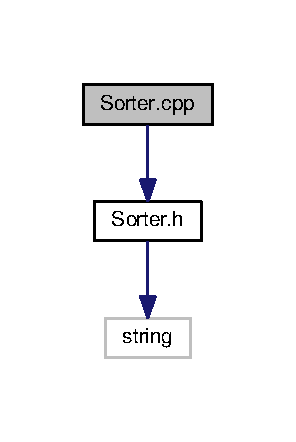
\includegraphics[width=186pt]{_sorter_8cpp__incl}
\end{center}
\end{figure}


\subsection{Detailed Description}
Implementation file for basic sorting structures. 

\begin{DoxyAuthor}{Author}

\end{DoxyAuthor}

\hypertarget{_sorter_8h}{}\section{Sorter.\+h File Reference}
\label{_sorter_8h}\index{Sorter.\+h@{Sorter.\+h}}


Declaration file for basic sorting structures.  


{\ttfamily \#include $<$string$>$}\\*
Include dependency graph for Sorter.\+h\+:
\nopagebreak
\begin{figure}[H]
\begin{center}
\leavevmode
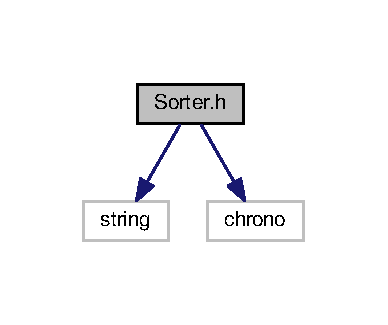
\includegraphics[width=131pt]{_sorter_8h__incl}
\end{center}
\end{figure}
This graph shows which files directly or indirectly include this file\+:
\nopagebreak
\begin{figure}[H]
\begin{center}
\leavevmode
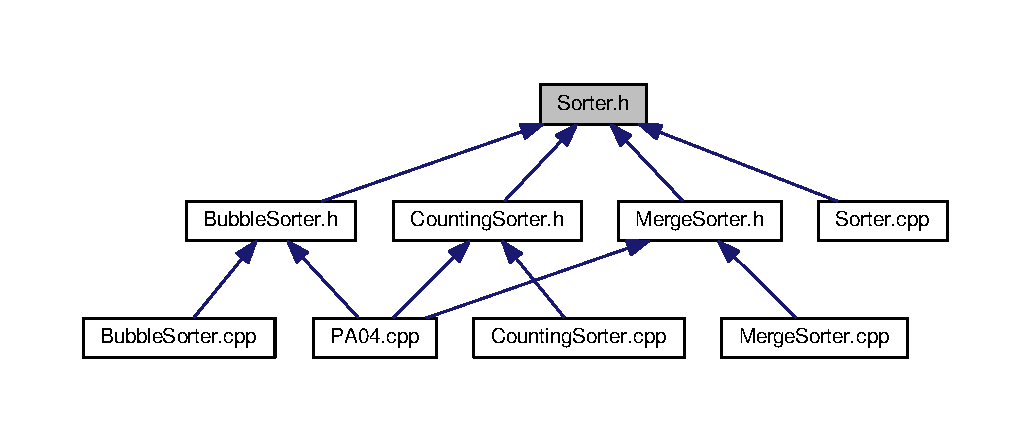
\includegraphics[width=350pt]{_sorter_8h__dep__incl}
\end{center}
\end{figure}
\subsection*{Classes}
\begin{DoxyCompactItemize}
\item 
struct \hyperlink{struct_sort_stats}{Sort\+Stats}
\begin{DoxyCompactList}\small\item\em Contains sorting statistics. \end{DoxyCompactList}\item 
class \hyperlink{class_sorter}{Sorter}
\begin{DoxyCompactList}\small\item\em Base class for \hyperlink{class_sorter}{Sorter} classes, which sort int data. \end{DoxyCompactList}\end{DoxyCompactItemize}


\subsection{Detailed Description}
Declaration file for basic sorting structures. 

\begin{DoxyAuthor}{Author}
Matthew Bauer 
\end{DoxyAuthor}

%--- End generated contents ---

% Index
\backmatter
\newpage
\phantomsection
\clearemptydoublepage
\addcontentsline{toc}{chapter}{Index}
\printindex

\end{document}
